\documentclass{beamer}
\usepackage{polski}
\usepackage[utf8]{inputenc}
\usepackage{pgfplotstable}
\usepackage{pgfplots}
\usepackage{graphicx}

\useoutertheme{infolines}

\usetikzlibrary{calc}
\pgfplotsset{compat=1.5}
\usetheme{Warsaw}

\setbeamercovered{transparent}

\author {Karol Olko, Tomasz Pasternak,\\ Rafał Kułaga, Michał Jędros}
\title {Spiking Neural Networks}
\begin{document}
\frame{\titlepage}
\frame{\tableofcontents}

\section{Budowa sieci}

\begin{frame}
  \begin{block}{Podejście tradycyjne}
    \begin{itemize}
    \item Bierzemy pod uwagę jedynie częstotliwość wysyłania impulsów jako nośnik informacji między neuronami
    \item Duże straty informacji
    \end{itemize}
  \end{block}
\end{frame}
\begin{frame}
  \begin{block}{Podejście impulsowe}
    \begin{itemize}
    \item<1-> Czas wyjścia każdego impulsu jest brany pod uwagę
    \item<2-> O stanie wyjściowym neuronu może decydować kolejność impulsów
    \item<3-> Wierniejsze odwzorowanie biologicznych NN
    \item<4-> Wymagana większa moc obliczeniowa
    \end{itemize}
  \end{block}
\end{frame}

\begin{frame}
  \begin{block}{Założenia modelu impulsowego}
    \begin{itemize}
    \item Jedno wejście - wiele wyjść
    \item Prawdopodobieństwo ``strzału'' rośnie z czasem
    \item Dynamika opisana przez conajmniej jedną zmienną
    \end{itemize}
  \end{block}
\end{frame}

\begin{frame}
  \begin{center}
    \begin{tikzpicture}
      \begin{axis}[name = neuron1, title=Neuron 1, height=3cm, width=10cm]
        \addplot[blue] table {neuron1.dat};
      \end{axis}
      \begin{axis}[name = neuron2, title=Neuron 2, at={($(neuron1.south west)-(0,2cm)$)}, height=3cm, width=10cm, anchor=west]
        \addplot[blue] table {neuron2.dat};
      \end{axis}
    \end{tikzpicture}
  \end{center}
  Neuron posiadający neurony wejściowe wysyłające takie sygnały może zachować się inaczej, gdy przyjmiemy podejście impulsowe.
\end{frame}

\subsection{Model impulsowy}
\begin{frame}
  \begin{block}{Model LIF (Leaky Integrate-and-Fire) \cite{Ponulak2011}}
    $$ C\frac{\mathrm{d}u}{\mathrm{d}t} (t) = -\frac1Ru(t)+\left(i_0(t) + \sum{w_ji_j(t)}\right)$$ 
    $u(t)$ -- zmienna stanu \\ 
    $C$ -- pojemność membrany \\
    $R$ -- rezystancja wejściowa\\
    $i_0(t)$ -- zewnętrzny prąd \\
    $i_j(t)$ -- wejście z $j$-tego połączenia synaptycznego\\
    $w_j$ -- waga $j$-tej synapsy
  \end{block}
\end{frame}
\subsection{Topologie}
\subsubsection{Feedforward}
\begin{frame}{Feedforward}
\begin{itemize}
	\item Przepływ sygnału jednokierunkowy, brak sprzężenia zwrotnego
	\item Modelowanie prostych receptorów, np. wzroku \cite{Perrinet2004}, smaku, dotyku. 
\end{itemize}
\end{frame}
\subsubsection{Rekurencyjna}
\begin{frame}{Rekurencyjna}
\begin{itemize}
	\item Istnienie wzajemnych połączeń między neuronami - sieci ze stanem
	\item Większe możliwości obliczeniowe, trudniejsza kontrola i uczenie
	\item Wykorzystywane m.in. do modelowania procesów decyzyjnych w mózgu \cite{Wang2008} a także dynamiki układów wzajemnie zależnych (modelowanie oscylacji sieci)
\end{itemize}
\end{frame}
\subsubsection{Hybrydowa}
\begin{frame}{Hybrydowa}
\begin{itemize}
	\item Sieć z częścią populacji o topologii feed-forward, reszta - rekurencyjne
	\item Interakcje między populacjami - jednokierunkowe lub wzajemne
	\item Modelowanie procesu uczenia (\textit{synfire chain})
	\item Uczenie rezerwuarowe
\end{itemize}
\end{frame}
\section{Kodowanie informacji}
\subsection{Częstotliwość sygnałów a modele zależne od czasu}
\begin{frame}
\begin{itemize}
 	\item Ilość informacji możliwych do zakodowania
 	\item Rozróżnianie sekwencji sygnałów
 	\item Rozdzielczość
\end{itemize}
\end{frame}
\subsection{Przykłady kodowania sygnałów w SNN}
\begin{frame}{Time-to-first-spike}
	\begin{figure}[ht]
		\begin{minipage}{0.48\linewidth}
			\begin{itemize}
				\item Prostota
				\item Szybkość
				\item Sygnał niesie dostatecznie dużo informacji, by zakodować dane pochodzące z receptorów czuciowych na opuszkach palców
			\end{itemize}
		\end{minipage}
		\hfill
		\begin{minipage}{0.48\linewidth}
		\centering
		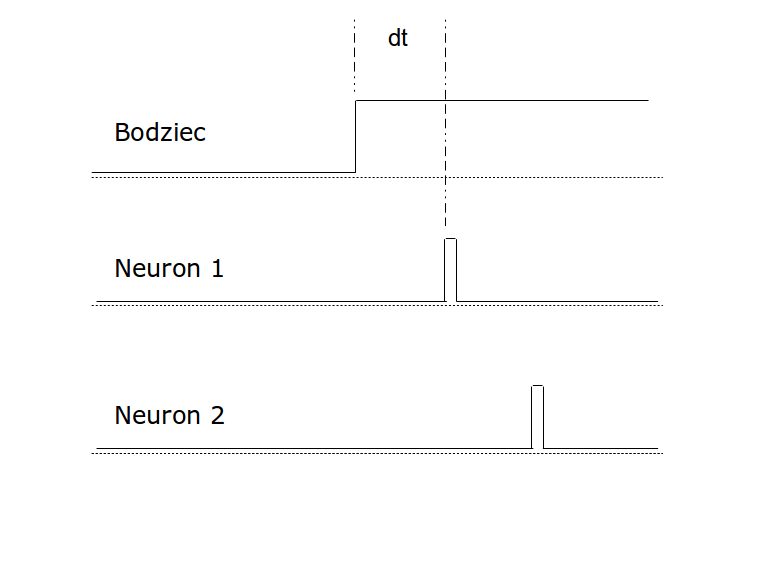
\includegraphics[width=\textwidth]{TimeToFirstSpike.png}
		\caption{Czas najszybszej odpowiedzi}
		\end{minipage}
	\end{figure}
\end{frame}

\begin{frame}{Rank-order coding}
	\begin{figure}[ht]
		\begin{minipage}{0.48\linewidth}
			\begin{itemize}
				\item Informacja zakodowana przez kolejność przybytych sygnałów
				\item Proponowany model kategoryzacji zmysłu wzroku
			\end{itemize}
		\end{minipage}
		\hfill
		\begin{minipage}{0.48\linewidth}
		\centering
		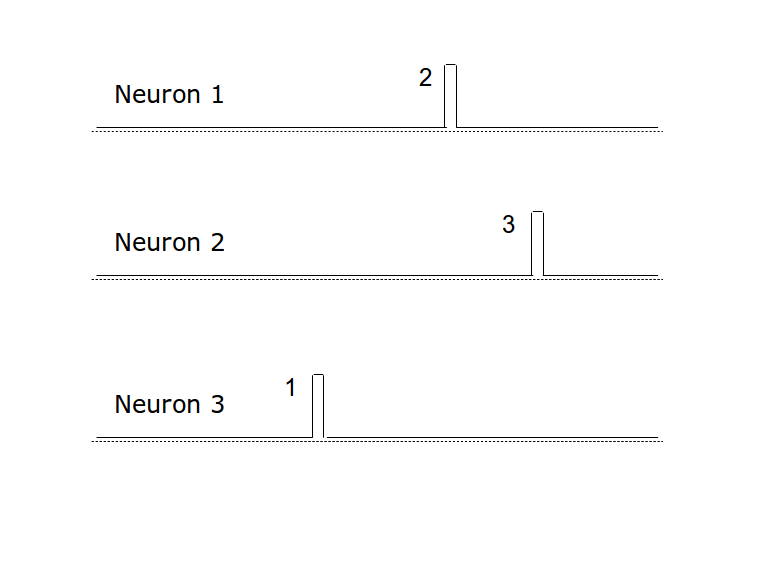
\includegraphics[width=\textwidth]{ROC.png}
		\caption{Kodowanie kolejnością przybycia sygnałów}
		\end{minipage}
	\end{figure}
\end{frame}


\begin{frame}{Latency code}
	\begin{figure}[ht]
		\begin{minipage}{0.48\linewidth}
			\begin{itemize}
				\item Przenoszenie informacji przez względny timing między impulsami
				\item Zdolność przenoszenia ogromnej ilości danych
			\end{itemize}
		\end{minipage}
		\hfill
		\begin{minipage}{0.48\linewidth}
		\centering
		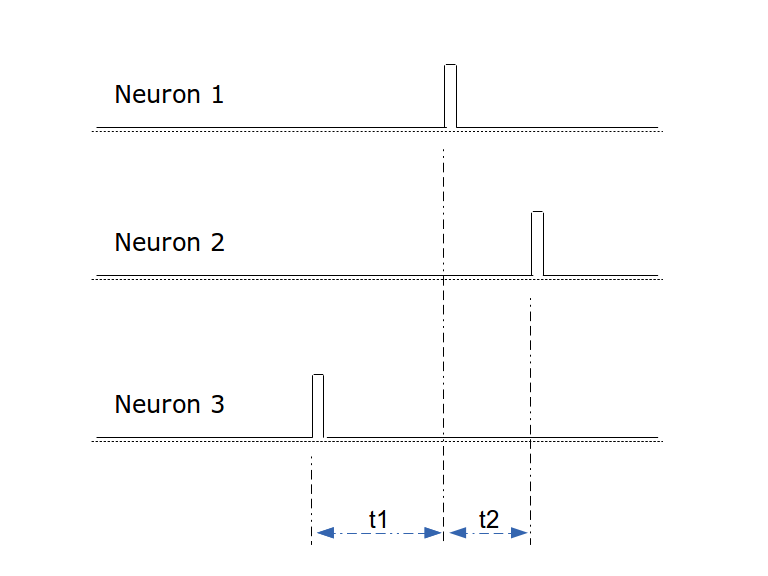
\includegraphics[width=\textwidth]{Latency.png}
		\caption{Względne opóźnienie impulsów}
		\end{minipage}
	\end{figure}
\end{frame}

\begin{frame}{Resonant burst model}
	\begin{figure}[ht]
		\begin{minipage}{0.48\linewidth}
			\begin{itemize}
				\item Odpowiednik filtra pasmowego
				\item Efektywna komunikacja między neuronami
			\end{itemize}
		\end{minipage}
		\hfill
		\begin{minipage}{0.48\linewidth}
		\centering
		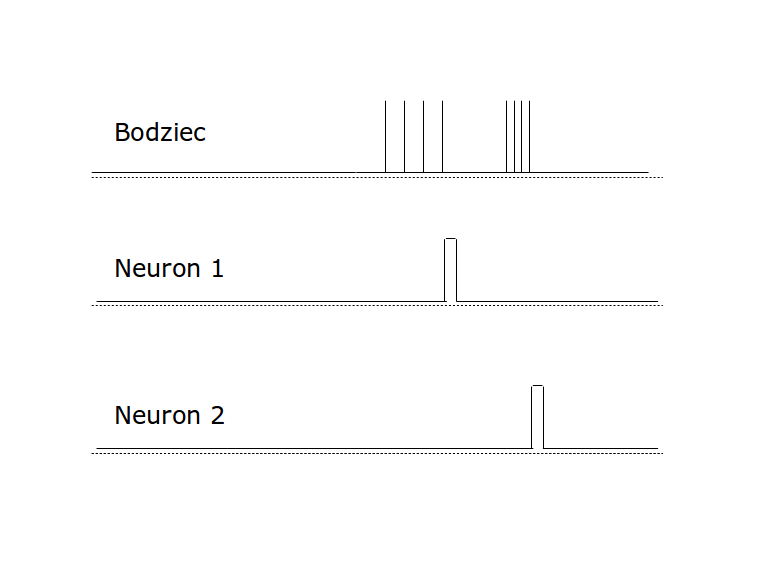
\includegraphics[width=\textwidth]{ResonantBurst.png}
		\caption{Sieć rezonansowa}
		\end{minipage}
	\end{figure}
\end{frame}

\begin{frame}{Coding by synchrony}
	\begin{figure}[ht]
		\begin{minipage}{0.48\linewidth}
			\begin{itemize}
				\item Teza: neurony kodujące różne bity informacji o tym samym obiekcie odpowiadają jednocześnie
				\item Przenoszenie bodźców istotnych dla całego organizmu
				\item Pakietowanie danych
			\end{itemize}
		\end{minipage}
		\hfill
		\begin{minipage}{0.48\linewidth}
		\centering
		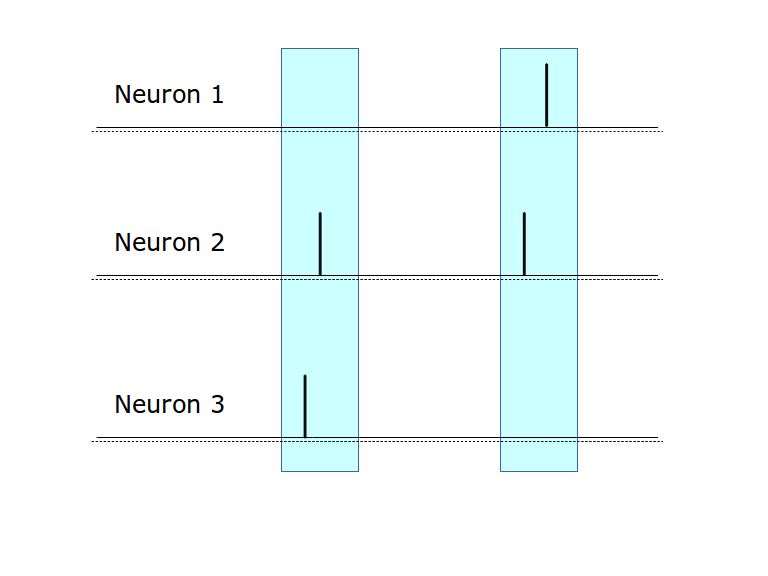
\includegraphics[width=\textwidth]{CodingBySynchrony.png}
		\caption{Kodowanie synchroniczne}
		\end{minipage}
	\end{figure}
\end{frame}

\begin{frame}{Phase Coding}
	\begin{figure}[ht]
		\begin{minipage}{0.48\linewidth}
			\begin{itemize}
				\item Czasy wyemitowanych impulsów są odniesione do punktu referencyjnego sygnału okresowego
				\item Przenoszenie informacji w obecności oscylacyjnego szumu
			\end{itemize}
		\end{minipage}
		\hfill
		\begin{minipage}{0.48\linewidth}
		\centering
		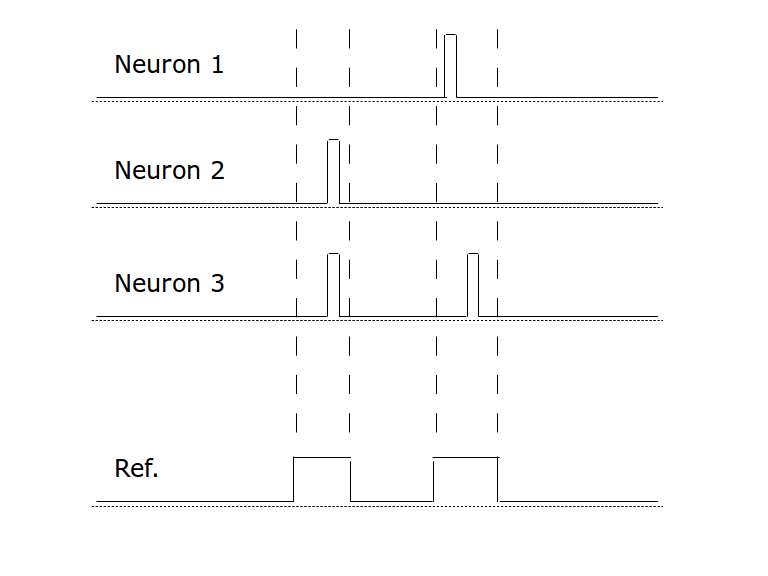
\includegraphics[width=\textwidth]{Phase.png}
		\caption{Kodowanie fazą}
		\end{minipage}
	\end{figure}
\end{frame}

\section{Uczenie}
\begin{frame}{Uczenie bez nadzoru}
	\begin{figure}[ht]
		\begin{minipage}{0.48\linewidth}
			\begin{itemize}
				\item Proces Hebba w klasycznym ujęciu: $\Delta w_{ij} = v_i v_j$
				\item Wpływ zależności czasowych między impulsami pre- i postsynaptycznymi na rodzaj pobudzenia: \newline \textbf{STDP} - \textit{Spike-Timing-Dependent-Plasticity}
				\item Model adaptacji neuronów zależnych od czasu impulsów: $\frac{d}{dt} w_{ji}(t) = a_0 + a_1 S_i(t) + a_2 S_j(t) + a_3 S_i(t) \overline{S_j}(t) + a_4 \overline{S_i}(t)S_j(t)$
			\end{itemize}
		\end{minipage}
		\hfill
		\begin{minipage}{0.48\linewidth}
		\centering
		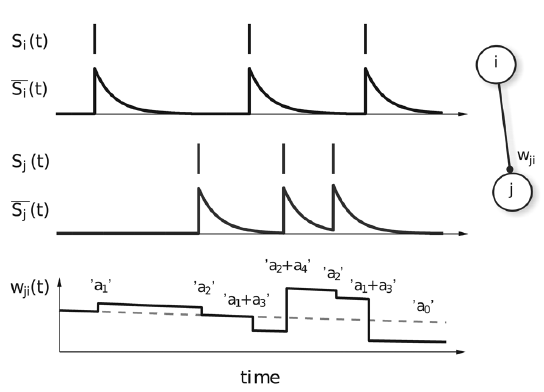
\includegraphics[width=\textwidth]{STDP.png}
		\caption{Przykład funkcjonowania modelu STDP}
		\end{minipage}
	\end{figure}
\end{frame}

\begin{frame}{Uczenie z nadzorem - model jednowarstwowy}
\begin{itemize}
	\item Trudność w zrozumieniu procesu uczenia biologicznych sieci neuronowych o zależnościach czasowych
	\item Nadzorowane uczenie Hebba (\textbf{SHL} -- \textit{Supervised Hebbian Learning}) i jego ograniczenia
	\item Model uczenia \textbf{ReSuMe}: $\frac{d}{dt} w_{ji}(t) = a \left[S_d(t) - S_j(t) \right] \overline{S_i}(t)$, gdzie a - szybkość uczenia, $S_d$ - referencyjny ciąg impulsów, $S_j$ - odpowiedź sieci, $\overline{S_i}(t)$ - ciąg impulsów wejściowych, po użyciu filtra LP.
\end{itemize}
\end{frame}

\begin{frame}{Uczenie z nadzorem - model wielowarstwowy}
\begin{itemize}
	\item Trudność w implementacji algorytmu \textbf{BP}
	\item Algorytm \textbf{SpikeProp} i jego ograniczenia
\end{itemize}
\end{frame}

\begin{frame}{Reinforcement learning}

	\begin{figure}[ht]
		\begin{minipage}{0.48\linewidth}
			\begin{itemize}
				\item Uczenie w obecności sygnałów nagrody / kary
				\item Korelacja układu dopaminergicznego z sygnałami nagrody przewidzianymi teoretycznie
				\item $\frac{d}{dt}w_{ji}(t) = c_{ji}(t)d(t)$, gdzie $c_{ji}$ - podatność na zmianę wagi, d(t) - sygnał nagrody 
			\end{itemize}
		\end{minipage}
		\hfill
		\begin{minipage}{0.48\linewidth}
		\centering
		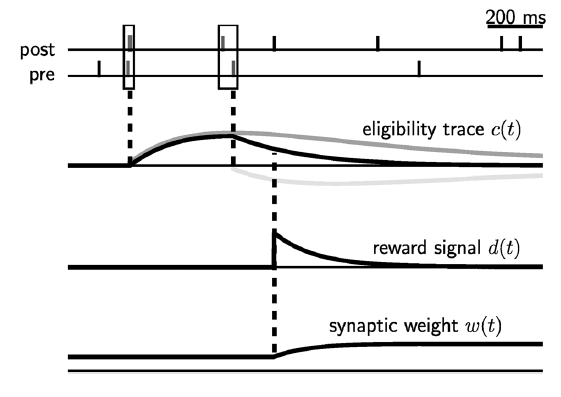
\includegraphics[width=\textwidth]{reinforcement.png}
		\caption{Przykład funkcjonowania modelu \textit{reinforcement learning}}
		\end{minipage}
	\end{figure}

\end{frame}

\section{SNN, a kora wzrokowa}
\begin{frame}{Wprowadzenie}
\begin{figure}[ht]

		\centering
		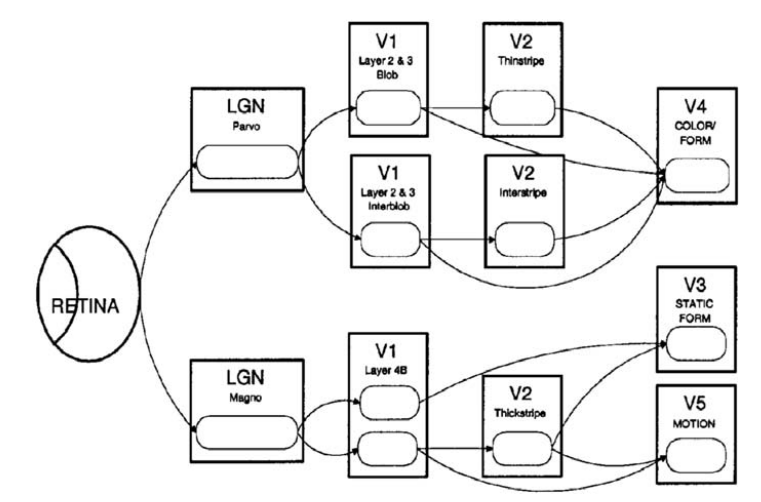
\includegraphics[width=0.7\textwidth]{visualSystemModel.png}
		\caption{Model systemu}

	\end{figure}
\end{frame}
\subsection{Modele}
\begin{frame}{Model Hodgkin-Huxley'a}
potencjał błonowy 
$$I=m^3 hG_{Na} (E-E_{Na}) + n^4G_K(E-E_K)+G_L(E-E_L) $$
\begin{itemize}
\item $I$ - prąd jonowy
\item $m$ - prawdopodobieństwo otwartego kanału
\item $G$ - przewodnictwo (Sód, Potas, upływ prądu)
\item $E$ - potencjał
\end{itemize}
\end{frame}
\begin{frame}{Model FitzHugh–Nagumo}
\begin{itemize}
\item Zachowanie neuronu jak oscylatora van der Pola. 
\item Połączone oscylacje dla każdego neuronu.
$$\varepsilon \frac{dx}{dt} = -y-g(x)+I$$

$$\frac{dy}{dt} = x -by$$
\item $g(x)=x(x-a)(x-1),0<a<1$ 
\item $I$ -prąd wejściowy
\item $\varepsilon<<1$
\item Opisane neurony możliwe do użycia w innych modelach biologicznych.
\item Każdy neuron to 2 połączone oscylacje połączone do innego neuronu.
\end {itemize}
\end {frame}
\begin {frame}
\begin{figure}[ht]
	\begin{minipage}{0.48\linewidth}
	\centering
	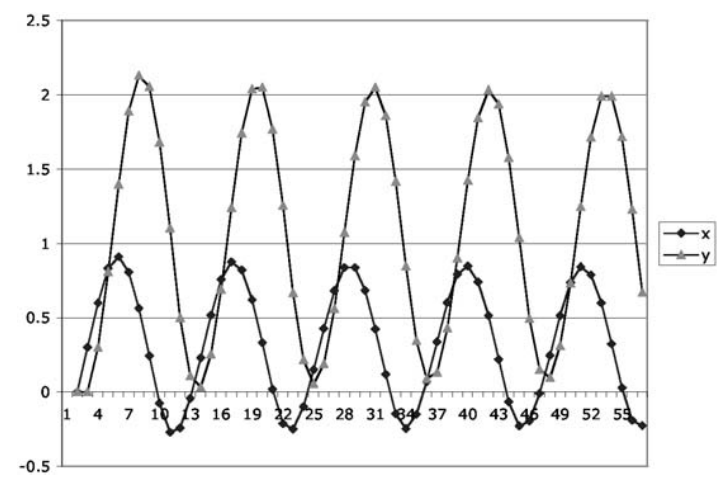
\includegraphics[width=\textwidth]{OscillatoryFN.png}
	\caption{Przedstawienie systemu oscylacyjnego na podstawie FitzHugh-Nagumo}
	\end{minipage}
\end{figure}
\begin{itemize}
\item Po zmianie parametrów a, b i I można otrzymać stan stabilny
\end{itemize}
\end{frame}
\begin{frame}{Model Eckhorna}
\begin{figure}[ht]
	\begin{minipage}{0.48\linewidth}
	\centering
	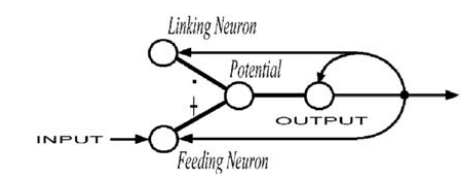
\includegraphics[width=\textwidth]{EckhornNeuron.png}
	\caption{Neuron typu Eckhorna}
	\end{minipage}
\end{figure}
\begin{itemize}
\item Na podstawie kory kota
\item Karmienie - impuls zewnętrzny i wewnętrzny
\item Skojarzenie - impuls wewnętrzny
\item $U_m$ - równanie drugiego rzędu, porównane do progu
\item Na wejście również od sąsiadów
\end{itemize}
\end{frame}
\begin{frame}
Sieć neuronowa połączonych impulsów
\begin{figure}[ht]
	\centering
	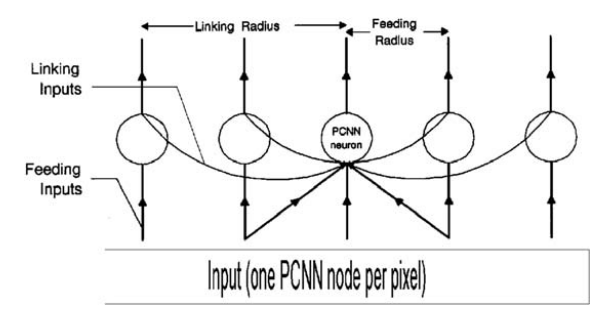
\includegraphics[width=0.85\textwidth]{PCNN.png}
	\caption{Neuron typu Eckhorna}
\end{figure}
\end{frame}

\begin{frame}{Model Rybaka}
\begin{itemize}
\item Na podstawie kory świnki morskiej
\item Bardzo podobne do Eckhorna
\item Dwa porównania- $X$ i $Z$ z bodźcem $S$
\item Nieliniowa funkcja progowa
\end{itemize}
\end{frame}

\begin{frame}{Model Parodi}
\begin{itemize}
\item Alternatywa dla modelu Eckhorna
\item Zwraca uwagę na brak synchronizacji
\item Zauważył podobieństwo wyjść elementów ruchomych i statycznych
\item Wprowadza opóźnienie przy synapsach
\item Reset neuronów
\end{itemize}
\end{frame}

\section{Zastosowania}

\begin{frame}{Zastosowania sieci impulsowych}

\begin{itemize}
\item Zastosowania sieci zależą od użytych metod uczenia
\item Na bazie koncepcji SNN powstało wiele interesujących implementacji sprzętowo-programowych (tzw. neurokomputerów)
\item Uważa się, iż analiza właściwości bardzo dużych sieci SNN, zaimplementowanych sprzętowo, może przynieść pewne odkrycia w dziedzinie mechanizmów działania mózgu
\end{itemize}

\end{frame}

\subsection{Sieci uczone bez nauczyciela}

\begin{frame}{Zastosowania sieci SNN uczonych bez nauczyciela (met. Hebba)}

\begin{itemize}
\item Samoorganizujące się mapy
\item Rozpoznawanie szeregów czasowych 
\item Pamięci asocjacyjne
\item Wyznaczanie głównych składowych ciągu impulsów
\end{itemize}

\end{frame}

\begin{frame}{Klasyfikacja}

\begin{itemize}
\item Sieci SNN nadają się do klasyfikacji rzeczywistych zestawów danych -- testy na typowych bazach danych: Iris, Wisconsin Breast Cancer itp.
\item Przykładem może być dwuwarstwową sieć feedforward używana do klasteryzacji i klasyfikacji. Implementuje ona modele lokalnych pól receptorowych łączących własności funkcji radialnych (RBF) i sieci SNN do konwersji sygnałów wejściowych (klasyfikowanych danych) w postaci zmiennoprzecinkowej do reprezentacji impulsowej. Wykorzystana metoda uczenia bazuje na metodzie Hebba i umożliwia separację złożonych klastrów poprzez synchronizację neuronów kodujących różne części klastra danych. Wynik klasyfikacji komunikowany jest na dwa sposoby: aktywny neuron oznacza wynik klasyfikacji (klasę), zaś czas jego zadziałania -- odległość pomiędzy danymi wejściowymi a środkiem klastru.
\end{itemize}

\end{frame}

\begin{frame}{Rozpoznawanie obrazów}

\begin{itemize}
\item Sieć feedforward z uczeniem STDP i kodowaniem rank-order umożliwia szybkie rozpoznawanie obrazów. Sieć taka składa się z dwóch warstw neuronów. W każdym kroku uczenia, jeden z obrazów podawany jest na wejścia sieci. Prezentacja ta powoduje wyzwolenie pojedynczego impulsu w każdym neuronie pierwszej warstwy. Czasy wystąpienia impulsów są następnie delikatnie zaburzane, po czym dodawana jest Poissonowska aktywność spontaniczna. Sygnały wyjściowej pierwszej warstwy są następnie podawane na wejścia drugiej warstwy. Jej pierwszy aktywny neuron powoduję aktywację uczenia metodą STDP. W wyniku tego, jeden neuron uczy się tylko jednego wzorca. 
\end{itemize}

\end{frame}

\begin{frame}{Rozpoznawanie zapachów}

\begin{itemize}

\item W jednym z eksperymentów w SNN zamodelowane zostało działanie części mózgu owada, odpowiadającej za przetwarzanie bodźców zapachowych. Sieć ta została następnie wykorzystana do sterowania mobilnym robotem, w sposób powodujący nadążanie za źródłem zapachu. W użytym modelu, pobudzenie kodowane było za pomocą grupy kwazi-synchronicznych neuronów rzutujących, z których każdy działał na zasadzie pętli fazowej z lokalnymi oscylacjami. Adaptacja częstotliwości została użyta do czasowej ewolucji kodu przestrzennego, co miało na celu zwiększenie odległości pomiędzy podobnymi zapachami.

\end{itemize}

\end{frame}

\begin{frame}{Nawigacja przestrzenna i eksploracja środowiska}

\begin{itemize}

\item Przy pomocy sieci impulsowych modeluje się również działanie ośrodków odpowiedzialnych za tworzenie map otoczenia i planowanie ruchów, zlokalizowanych w hipokampie. Sieć taka składa się z komórek reprezentujących miejsca (\emph{place cells}), połączonych na zasadzie każdy-z-każdym. Poszczególne komórki aktywowane są w momencie wkroczenia w obszar przez nie reprezentowany. Połączenia odpowiadające obszarom odwiedzanym zaraz po sobie są wzmacniane, co znajduje później zastosowanie do planowania ruchów -- w komórce odpowiadającej aktualnemu położeniu obiektu inicjalizowane jest pobudzenie, które przekazane zostaje do pozostałych komórek sieci. Pobudzenie to jest tym silniejsze, im "bliżej" siebie zlokalizowane są poszczególne obszary. Sygnał wędruje najmocniejszymi połączeniami, aż do osiągnięcia zadanego celu (obszaru docelowego).

\end{itemize}

\end{frame}


\subsection{Sieci uczone z nauczycielem}

\begin{frame}{Zastosowania sieci SNN uczonych z nauczycielem}

\begin{itemize}

\item Serwomechanizmy i planowanie ruchu
\item Klasyfikacja danych 
\item Podejmowanie decyzji, z aplikacjami dla rynków finansowych

\end{itemize}

\end{frame}

\subsection{Sieci uczone metodą reinforcement learning}

\begin{frame}{Zastosowania sieci SNN uczonych metodą reinforcement learning}

\begin{itemize}

\item Nawigacja przestrzenna i planowanie ruchu
\item Podejmowanie decyzji
\item Eksperymentalne modele kardiostymulatorów

\end{itemize}

\end{frame}


\begin{frame}{Nawigacja w labiryncie wodnym}

\begin{figure}[H]
  \centering
    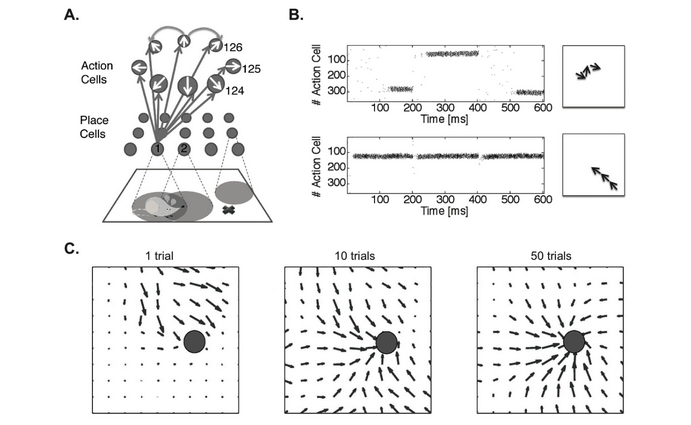
\includegraphics[width=0.85\textwidth]{water_maze.png}
\end{figure}

\end{frame}


\begin{frame}{Eksperymentalny kardiostymulator neuronowy}

\begin{itemize}

\item Rolą impulsowej sieci neuronowej w eksperymentalnym kardiostymulatorze jest dynamiczna optymalizacja odstępów czasowych pomiędzy pobudzeniami. 
\item Kardiostymulator taki działa w trybie master-slave -- procesor nadrzędny określa dopuszczalne tryby pracy, które uwzględniane są przy generowaniu pobudzeń.

\end{itemize}

\end{frame}


\begin{frame}{Eksperymentalny kardiostymulator neuronowy}

\begin{itemize}
\item Warstwy sieci i ich zadania:
\begin{itemize}

\item W warstwie wejściowej różne grupy synaps są pobudzane w zależności od średniej częstotliwości skurczy mięśnia sercowego. W każdej z grup każda synapsa jest pobudzana z pewnym ustalonym i rosnącym opóźnieniem od synchronizującego zdarzenia przedsionkowego. 
\item Druga warstwa sieci uczona jest z zastosowaniem metody Hebba z sygnałami nagrody/kary i ma za zadanie określić optymalne interwały pomiędzy sygnałami wyzwalającymi stymulację.
\item Warstwa wyjściowa sieci składa się z dwóch zestawów neuronów LIF, które sumują odpowiedzi neuronów warstw wcześniejszych i określają stymulację obu komór.

\end{itemize}
\end{itemize}

\end{frame}

\subsection{SpiNNaker}

\begin{frame}{Superkomputer neuronowy SpiNNaker}

\begin{itemize}

\item Masywnie równoległy komputer neuromorficzny, budowany obecnie na Manchester University w Wielkiej Brytanii

\item Jego zadaniem jest modelowanie bardzo dużych (biologicznie realistycznych) impulsowych sieci neuronowych w czasie rzeczywistym

\item System ten stanie się platformą do badania rozmaitych algorytmów i typów impulsowych sieci neuronowych

\end{itemize}

\end{frame}

\begin{frame}{Architektura sprzętowa}

\begin{itemize}

\item 65,536 identycznych, 18-rdzeniowych procesorów, co daje 1,178,648 rdzeni ARM968 taktowanych zegarem 200 MHz
\item Każdy z procesorów ma 128 MB pamięci, używanej do przechowywania wartości współczynników wagowych
\item Każdy z rdzeni posiada 32 kB pamięci instrukcji i 64 kB pamięci danych
\item Proces technologiczny 130 nm -- stosunkowo przestarzały (2012 -- 22 nm)
\item Pojedynczy rdzeń jest w stanie modelować działanie około tysiąca neuronów, co dla docelowego systemu umożliwi symulację około 1\% z wszystkich neuronów zawartych w mózgu

\end{itemize}


\end{frame}

\begin{frame}{Architektura sprzętowa}

\begin{figure}[H]
  \centering
    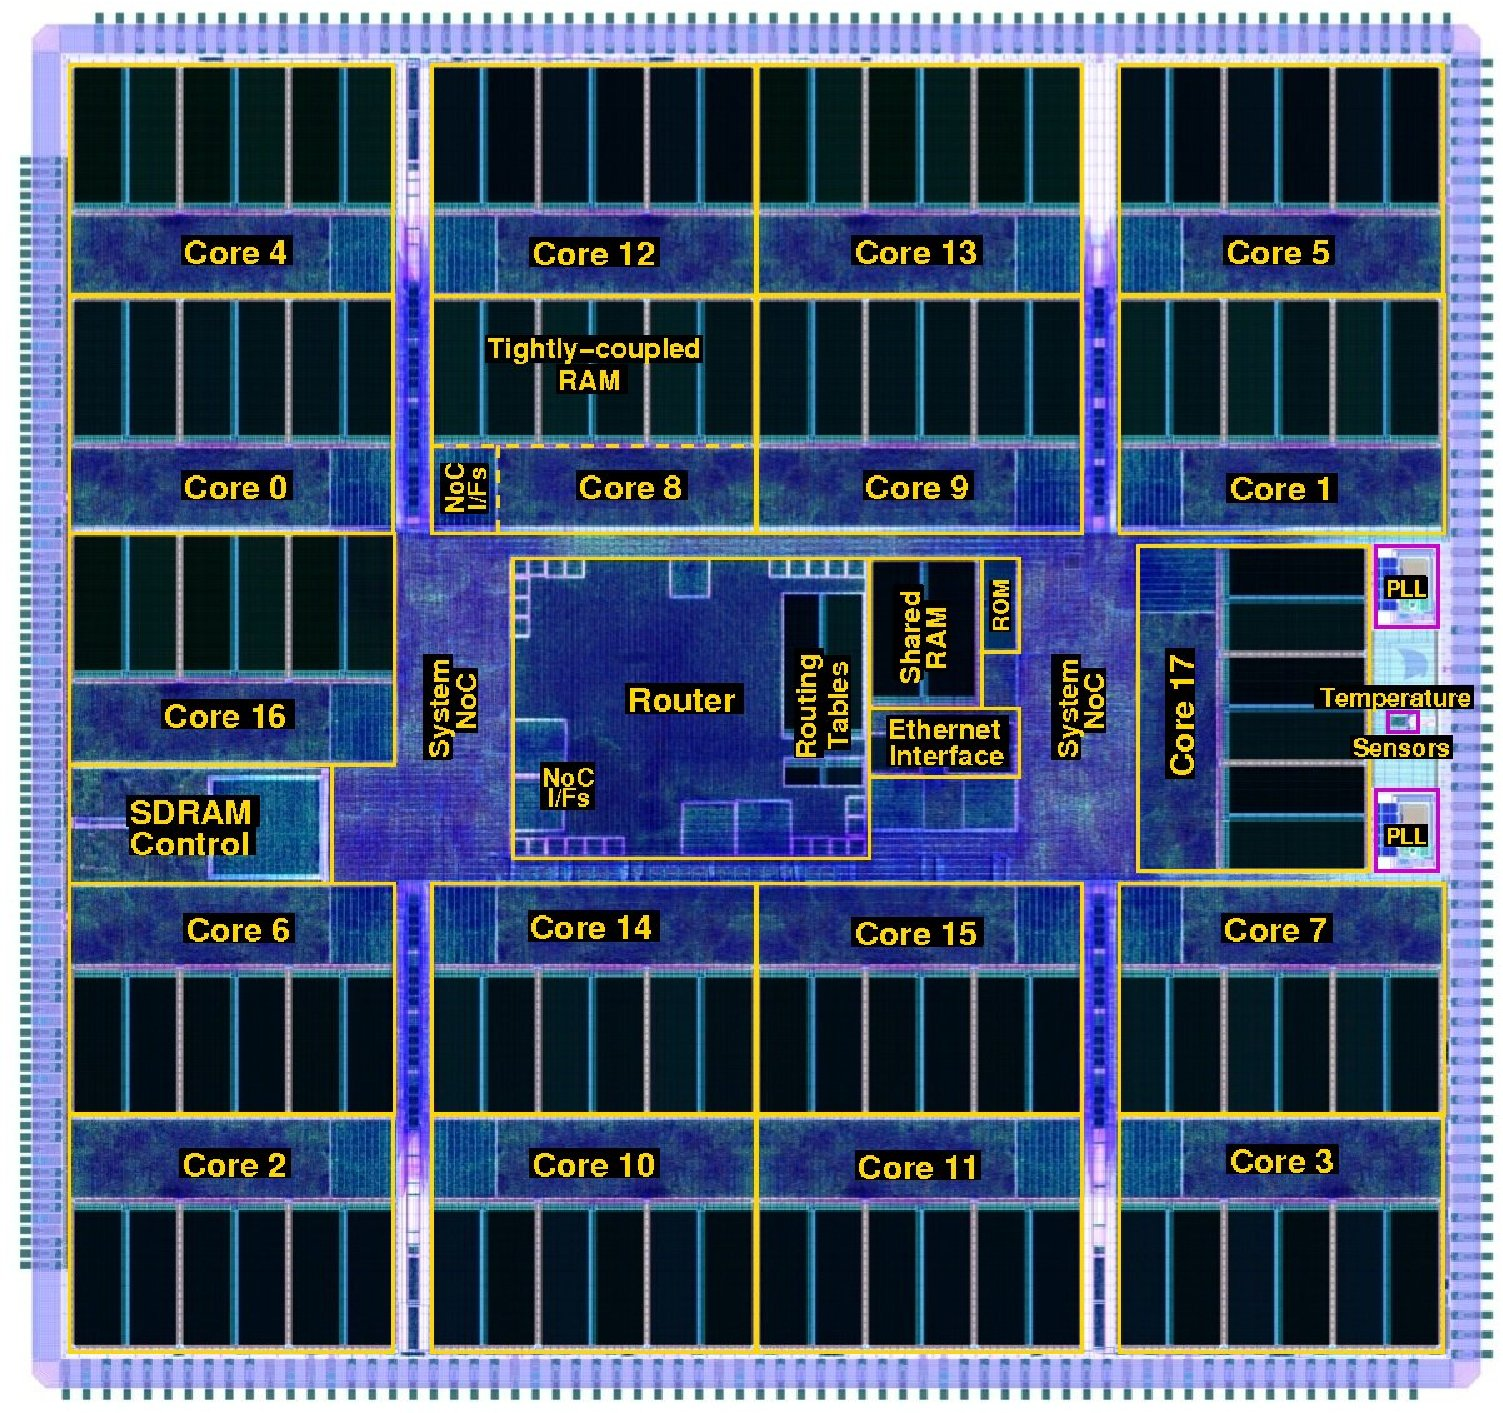
\includegraphics[width=0.5\textwidth]{spinnaker_chip.png}
\caption{Pojedynczy procesor systemu SpiNNaker}
\end{figure}

\end{frame}

\begin{frame}{Architektura sprzętowa}

\begin{figure}[H]
  \centering
    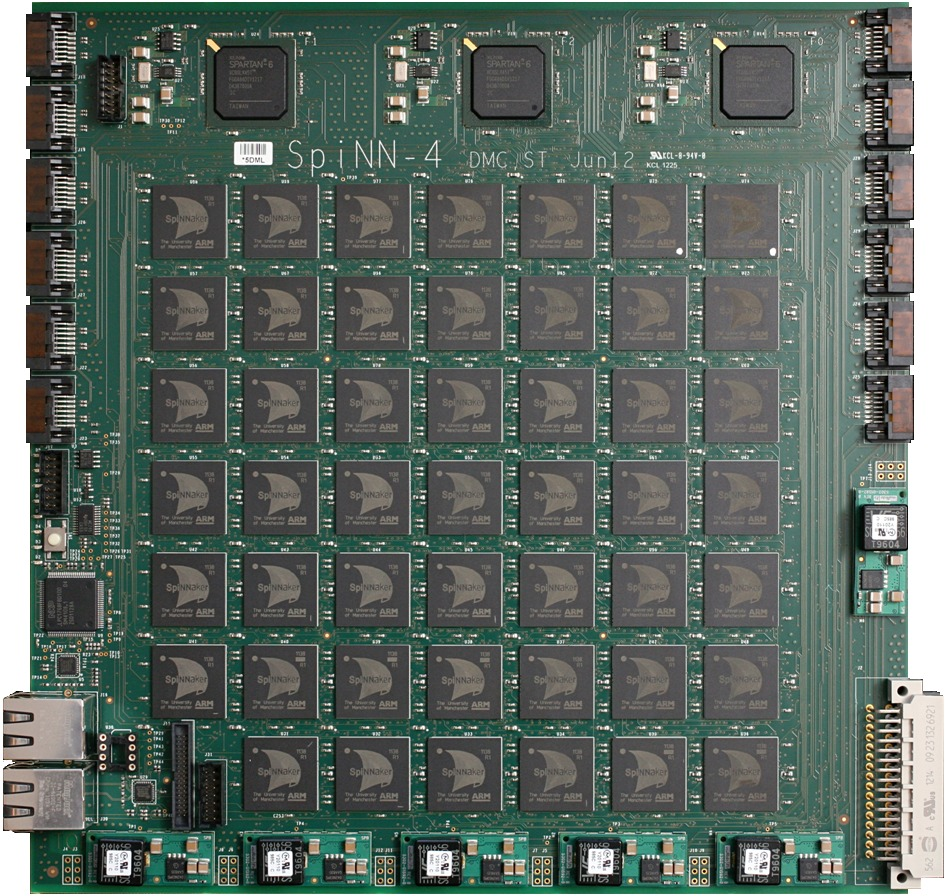
\includegraphics[width=0.5\textwidth]{spinnaker_pcb.jpg}
\caption{Moduł zawierający 48 procesorów SpiNNaker}
\end{figure}

\end{frame}


\begin{frame}{Architektura sprzętowa -- połączenia}

\begin{itemize}

\item Magistrale połączeniowe w pełni cyfrowe

\item Dowolna struktura połączeń

\item Niewielki rozmiar pakietów: 40/72 bity

\item Całkowita przepustowość -- 5,000,000 pakietów/sekundę

\item Mechanizmy wykrywania awarii poszczególnych procesorów i ich wyłączenia z sieci

\end{itemize}

\end{frame}



\begin{frame}{Pobór mocy}

\begin{itemize}

\item Ludzki mózg pobiera około 10 W energii

\item Docelowo, superkomputer SpiNNaker pobierać będzie 50-100 kW energii przy maksymalnym obciążeniu, przy symulacji 1\% wszystkich neuronów mózgu

\item Teoretyczna wydajność ludzkiego mózgu jest więc 500,000 razy większa

\end{itemize}

\end{frame}


\begin{frame}

\Huge{Dziękujemy za uwagę!}

\end{frame}



\section{Bibliografia}
\bibliographystyle{plain}
\bibliography{bibliografia}
\begin{frame}
\end{frame}

\end{document}
